\chapter{Proposta Experimental}
\label{chap:proposta}

%--------------------------------------------------------
\section{Materiais} 
\label{sec:cap5_materiais}

Esta seção visa trazer informações sobre tanto o \textit{hardware} quanto o \textit{software} utilizado nos experimentos para fins de reprodução. A Tabela. \ref{tab:hardware_software} referência tanto o \textit{hardware} como as principais bibliotecas utilizadas e suas versões.

\begin{table}[hbtp]
    \centering
    \renewcommand{\arraystretch}{1} % default é 1 
    % \begin{tabular}{|>{\centering\arraybackslash}p{2cm}|p{12cm}|}
    \begin{tabular}{|c|c|}
    \hline 
       \textbf{Item} & \textbf{Descrição}\\
    \hline 
       Computador & \textit{Macbook M1 Pro}  \\
    \hline 
       Memória & 16gb  \\
    \hline 
       Versão \textit{Python} & 3.11.0  \\
    \hline 
       Versão \textit{pyradiomics} & 3.0.1 \\
    \hline 
       Versão \textit{torch} & 2.2.1 \\
    \hline 
       Versão \textit{torchvision} & 0.17.1 \\
    \hline 
       Versão \textit{numpy} & 1.26.4 \\
    \hline 
       Versão \textit{scikit-learn} & 1.4.1.post1 \\
    \hline 
    \end{tabular} 
    \caption{Fonte: Autor}
    \label{tab:hardware_software}
\end{table}


%--------------------------------------------------------
\section{Conjunto de Dados} 
\label{sec:cap5_conj_dados}

Os experimentos foram  aplicados em duas bases distintas com imagens de RM do coração, informações a cerca do paciente e rótulos que indicam presença ou não de cardiomiopatia. O primeiro conjunto de dados é o \gls{ACDC} e consiste de dados públicos e são utilizados como linha de base para avaliação dos métodos aplicados. O segundo conjunto de dados consiste, de um conjunto de dados privado, seu acesso
se dá pela parceria existente entre o \gls{FEI} e o \gls{InCor}.

%--------------------------------------------------------
\subsection{Conjunto de Dados ACDC} 
\label{subsec:cap5_acdc}

O conjunto de dados \gls{ACDC} foi criado a partir de exames clínicos reais adquiridos no hospital universitário de Dijon (França). Os dados adquiridos foram totalmente anonimizados e tratados de acordo com as regulamentações estabelecidas pelo comitê ético local do hospital de Dijon. O conjunto de dados cobre várias patologias bem definidas com casos suficientes para (1) treinar adequadamente métodos de aprendizado de máquina e (2) avaliar claramente as variações dos principais parâmetros fisiológicos obtidos a partir de cine-RM (em particular volume diastólico e fração de ejeção). O conjunto de dados é composto por 150 exames (todos de pacientes diferentes) divididos em cinco subgrupos distribuídos de forma igualitária, sendo quatro patológicos e um grupo de sujeitos saudáveis. Dentre as cinco classes distintas, tem-se: \gls{DCM}, \gls{HCM}, \gls{NOR}, \gls{MINF} e \gls{RV}. As classes DCM e HCM são interpretadas como passíveis de \gls{CH} e as demais; NOR, MINF e RV; são interpretadas como o coração em condições normais, detalhes das classes podem ser verificados na Tabela \ref{tab:conditions}. 

\begin{table}[hbtp]
    \centering
    \renewcommand{\arraystretch}{1} % default é 1 
    \begin{tabular}{|>{\centering\arraybackslash}p{2cm}|p{12cm}|}
    \hline 
          % \textbf{Condição} & \textbf{Descrição} & Característica \\ 
          % \textbf{Condição} & \textbf{Descrição} \\ 
          \multicolumn{1}{|c|}{\textbf{Condição}} & \multicolumn{1}{c|}{\textbf{Descrição}} \\
          & \\
    \hline 
        \textbf{DCM} &
        A cardiomiopatia dilatada é uma condição em que o coração se 
        torna dilatado e não consegue bombear o sangue de forma
        eficiente. 
        \newline \newline
        \textbf{Característica}: O ventrículo esquerdo está dilatado e com função sistólica reduzida. \\ 
    \hline
        \textbf{HCM} & 
        A cardiomiopatia hipertrófica é uma condição onde há um espessamento anormal do músculo cardíaco, especialmente do ventrículo esquerdo. 
        \newline \newline
        \textbf{Característica}: A parede do ventrículo esquerdo está significativamente espessada, o que pode restringir o volume sanguíneo e o fluxo de saída. \\ 
    \hline
        \textbf{NOR} & 
        Esta classe representa corações normais sem qualquer condição patológica. 
        \newline \newline
        \textbf{Característica}: Estruturas e funções cardíacas normais, sem dilatações ou hipertrofias significativas. \\ 
    \hline
        \textbf{MINF} & 
        O infarto do miocárdio, ou ataque cardíaco, ocorre quando o fluxo sanguíneo para uma parte do coração é bloqueado por um período suficiente para causar danos ao músculo cardíaco. 
        \newline \newline
        \textbf{Característica}: Áreas do coração mostram cicatrizes ou fibrose devido ao infarto anterior, frequentemente visível nas imagens de ressonância magnética. \\ 
    \hline
        \textbf{RV} & 
        A hipertrofia do ventrículo direito é uma condição em que o ventrículo direito do coração está aumentado. 
        \newline \newline
        \textbf{Característica}: Espessamento da parede do ventrículo direito, que pode ser devido a diversas condições, como hipertensão pulmonar ou doenças congênitas do coração. \\
    \hline
    \end{tabular} 
    \caption{Fonte: Autor}
    \label{tab:conditions}
\end{table}


Os dados encontram-se balanceados e a distribuição dos dados pode ser conferida na Tabela. \ref{tab:count_dataset}. É possível notar, que após agrupamento das classes como especificado, estas tornam-se minimamente desbalanceadas, em uma proporção de 40/60.

Além disso, cada paciente vem com as seguintes informações adicionais: peso, altura, bem como os instantes das fases diastólica e sistólica \cite{bernardDeepLearningTechniques2018a}.

% DCM (Dilated Cardiomyopathy): This condition is characterized by an enlarged and weakened left ventricle that cannot pump blood efficiently. DCM can lead to heart failure and arrhythmias.

% HCM (Hypertrophic Cardiomyopathy): This is a genetic condition where the heart muscle (myocardium) becomes abnormally thick, which can make it harder for the heart to pump blood. It can also lead to problems with the heart's electrical system.

% NOR (Normal): This class represents individuals with normal cardiac function and no evident cardiac disease. These are typically healthy patients with no significant abnormalities in their heart structure or function.

% MINF (Myocardial Infarction): Commonly known as a heart attack, myocardial infarction occurs when blood flow to a part of the heart is blocked for a long enough time that part of the heart muscle is damaged or dies.

% RV (Right Ventricular Abnormality)

\begin{table}[hbtp]
    \centering
    \renewcommand{\arraystretch}{1} % default é 1 
    \begin{tabular}{|c|c|c|c|}
    \hline 
          \textbf{Grupo} & \textbf{Quantidade} & \textbf{C/ HC} & \textbf{S/ HC}  \\ 
    \hline 
        NOR & 30 & 0 & 30 \\ 
        DCM & 30 & 30 & 0\\ 
        HCM & 30 & 30 & 0\\ 
        MINF & 30 & 0 & 30 \\ 
        RV & 30 & 0 & 30 \\
    \hline 
        \textbf{Total}: & 150  & 60 & 90\\ 
    \hline 
    \end{tabular} 
    \caption{Fonte: Autor}
    \label{tab:count_dataset}
\end{table}

%--------------------------------------------------------
\subsection{Conjunto de Dados InCor} 
\label{subsec:cap5_incor}

O conjunto de dados \gls{InCor} é composto por casos reais de pacientes que realizaram exames de RMC e que foram classificados por especialistas do \gls{InCor} como casos que continham cardiomiopatia hipertrófica, cardiomiopatia dilatada ou nenhuma das duas anomalias. No total foram adquiridos 400 casos, distribuídos conforme a Figura \ref{fig:fig013}, na qual é possível verificar que a maioria dos casos (69\%) pertencem a indivíduos do sexo masculino, enquanto 31\% pertencem a mulheres. Dentro do grupo de homens verificou-se uma predominância de casos sem anomalia para pacientes com idades entre 21 a 41 anos (25\%), enquanto no grupo de mulheres notou-se que o número maior de casos (21\%) era composto por casos hipertróficos em pacientes com idade entre 42 a 62 anos \cite{bergamascoRECUPERACAOOBJETOSMEDICOS2018}.

\begin{figure}[htbp]
    \centering
    \caption{Distribuição das anomalias entre diferentes gêneros e idades}
    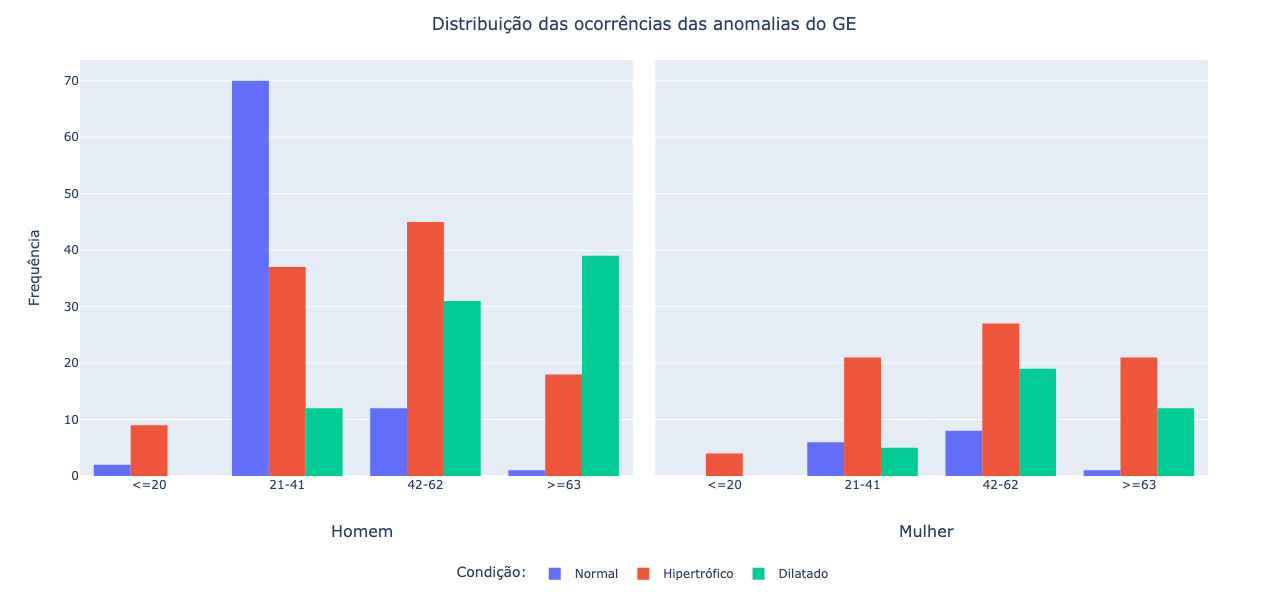
\includegraphics[width=1\textwidth]{figures/fig012.png}
    \caption*{Fonte: Autor}
    \label{fig:fig012}
\end{figure}

%--------------------------------------------------------
\subsection{Experimentos ACDC}
\label{subsec:cap5_experimentos_acdc}

Utilizando o conjunto de dados \gls{ACDC} como linha de base, foi utilizado os 100 exames de pacientes já previamente divididos, coletando apenas as fatias das imagens de RM apontadas como diástole junto com a máscara já disponível. \textit{Features} de primeira ordem e \gls{GLCM} são extraídas compondo ao todo 78 valores que compõem as features radiômicas. Para extração das \textit{features profundas}, é utilizada uma rede \textit{ResNet50} congelada é utilizada, a última camada densa é removida responsável por gerar a predição de 1000 classes, oriundas do conjunto de dados \textit{ImageNet}. A rede, após adaptada, passa a produzir 2048 \textit{features}.

A \textit{F-Test} é utilizado como seletor de \textit{features}, aplicado tanto nas \textit{features} radiômicas quanto nas profundas, as diminuindo ao valor de 64. Essas \textit{features} são concatenadas, e enviadas ao módulo de \textit{self-attention} e os resultados armazenados.

Neste experimento foi treinado o modelo utilizando, como função objetivo a entropia cruzada binária, taxa de aprendizado de $0,0001$, otimizador \textit{Adam}, tamanho de lote 4 e o treinamento se deu em aproximadamente 300 épocas, onde verificou que o erro se torna estável. Também foi empregada a estratégia de aleatorizar as entradas do modelo e descartar o último lote caso ele não alcance o tamanho especificado para o mesmo, neste caso 4. Com o resultado do modelo é aplicada a função sigmoide, Eq. \ref{eq:sigmoide}, função esta que limita os valores de seu resultado entre 0 e 1. Dos resultados, é classificado com CH todo valor $>0,5$ e normal o inverso.

\begin{equation}
\textit{sigmoide}(x) = \frac{1}{1 + e^x}
\label{eq:sigmoide}
\end{equation}

%--------------------------------------------------------
\section{Cronograma}
\label{sec:cronograma}

O cronograma proposto das atividades segue na Figura. \ref{fig:fig014}. De forma resumida, as disciplinas se encontram concluídas, resultados experimentais no conjunto de dados de base, \gls{ACDC} coletados e futuros experimentos arquiteturais em andamento.

\begin{figure}[htbp]
    \centering
    \caption{Cronograma planejado}
    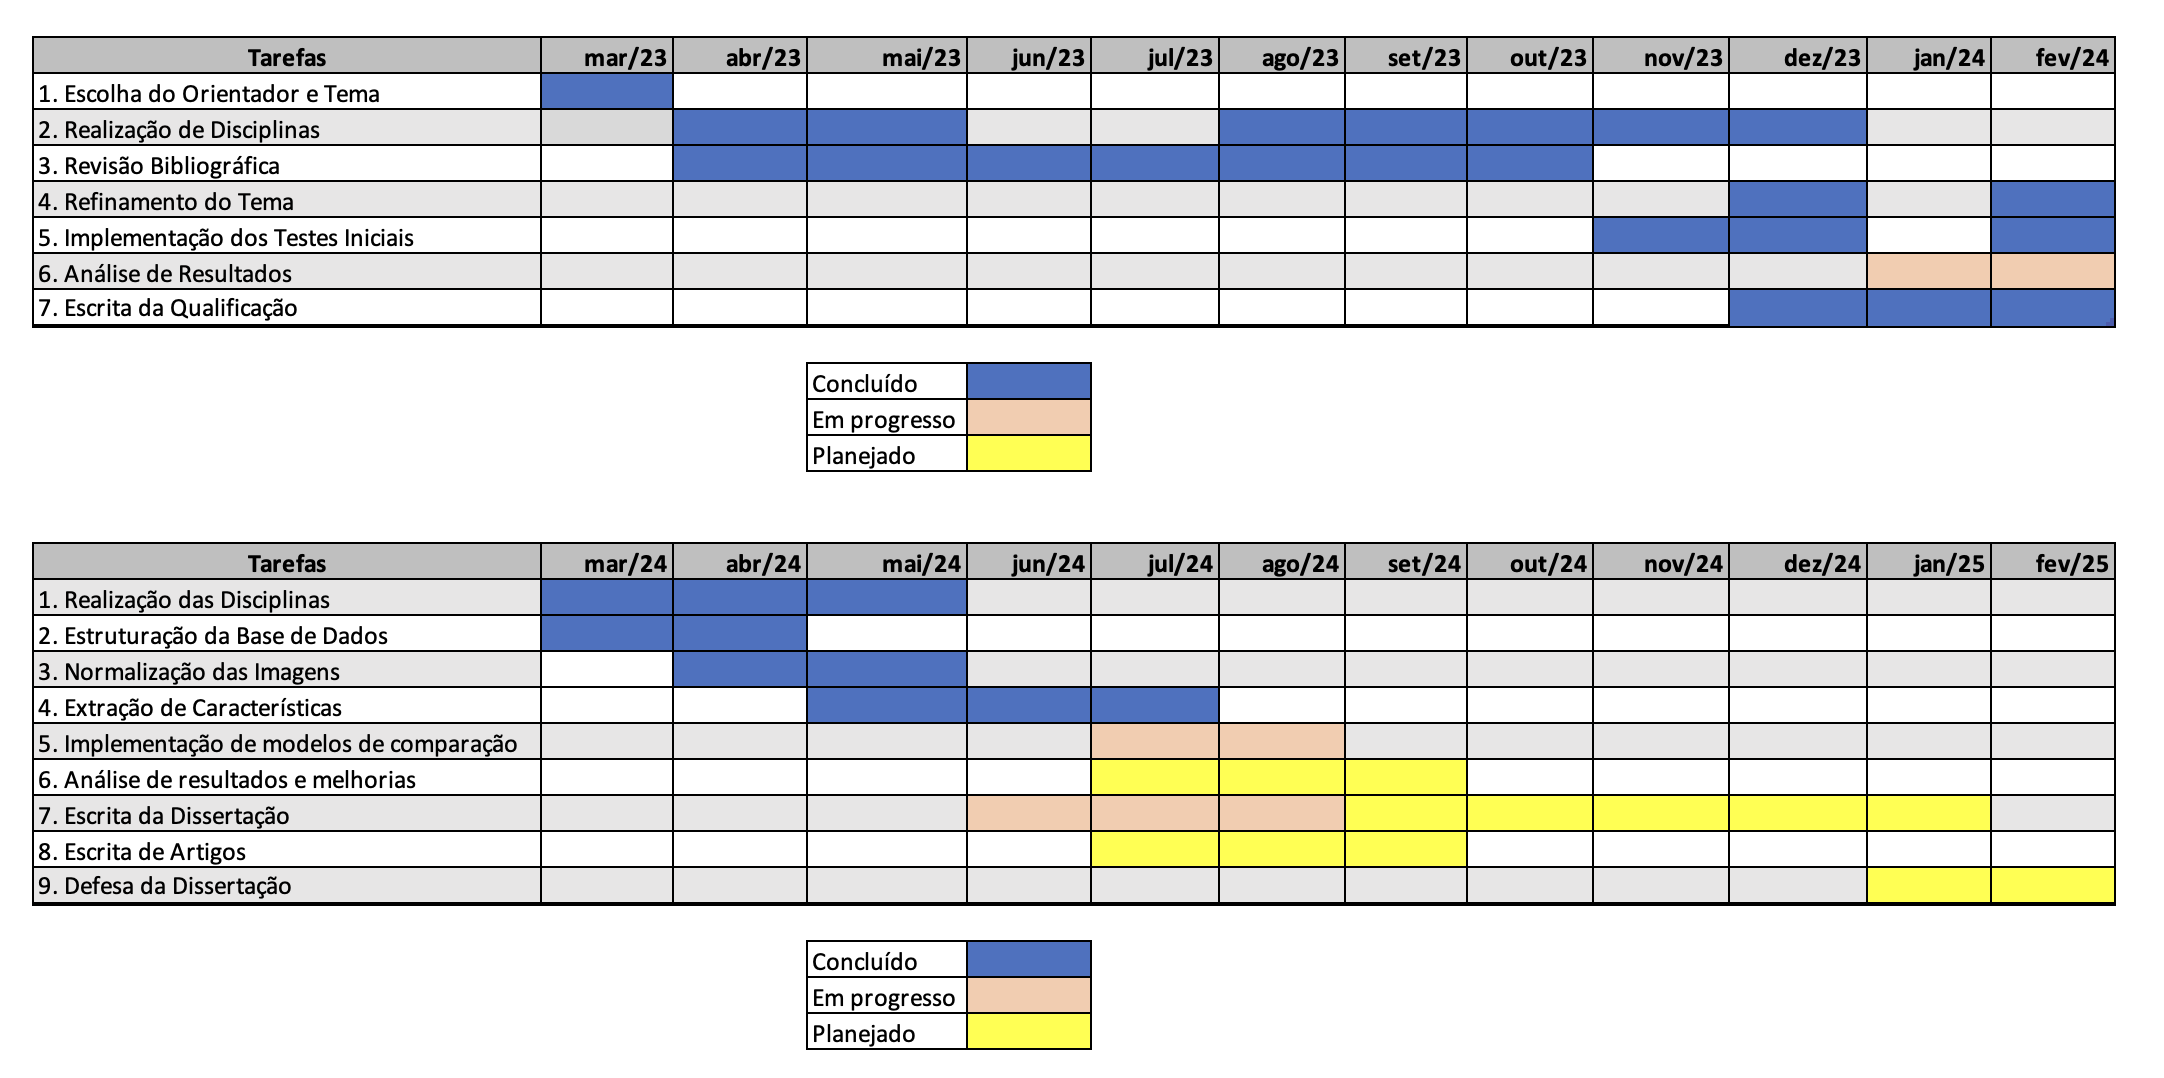
\includegraphics[width=1\textwidth]{figures/fig014.png}
    \caption*{Fonte: Autor}
    \label{fig:fig014}
\end{figure}
